\documentclass[11pt]{article}

%\input{macros}
\usepackage{amsmath,amssymb,graphicx}

\usepackage[hmargin=2cm,vmargin=2cm]{geometry}

\usepackage{ucs}
\usepackage[utf8x]{inputenc}
\usepackage{verbatim}

\usepackage{wrapfig}
\usepackage{subfig}
%\floatstyle{boxed} 
%\restylefloat{figure}

\newcommand{\eqb}{\begin{equation*}\begin{aligned}}
\newcommand{\eqe}{\end{aligned}\end{equation*}}
\newcommand{\eqnote}[1]{\text{\emph{#1}}}
\newcommand{\<}{\langle} 
\renewcommand{\>}{\rangle} 

\usepackage{tikz}
\usetikzlibrary{arrows,decorations.pathmorphing,backgrounds,positioning,fit,petri}

\makeatletter
\newcommand\paragraphnl{\@startsection{paragraph}{4}{\z@}%
  {-3.25ex\@plus -1ex \@minus -.2ex}%
  {1.5ex \@plus .2ex}%
  {\normalfont\normalsize\bfseries}}
\makeatother

%%%%%%%%%%%%%%%%%%%%%%%%%%%%%%%%%%%%%%%%%%%%%%%%%%%%%%%%%%%%%%%%%%%%%%%%
\author{Arthur Peters working with Nathan Collins}
\title{CS584: Project 1}
\date{\today}


\begin{document}
\maketitle

Our approach was to devise a translation from the given train network into a normal directed graph that describes all the states that the train can be in the network and which states can transition into which other states. Then we weight this graph appropriately to charge the correct costs for each problem. We can then use an unmodified shortest-path algorithm on this graph to find the path. 

\paragraph{A note on terminology:} I will refer to the train network given as the ``network'' and I will refer to the graph we transform it into as the ``graph''. The switches and end point on the network are collectively ``points'', and they are connected by ``segments.'' However the graph is made up of ``nodes'' (that represent states) and ``edges'' (that represent state transitions).

\section{Approach}

Before we do a true network to graph translation we do some clean up on the input network. This step produces a new network as output which contains no loop segments from a point to the same point. To do this we identify loops and split them into 2 segments with a new point in the middle. Note that this new point only has 2 segments attached to it so it is of a new kind which I will call a through point. The new segment and point and numbered with new IDs. We call these added points and segments ``phantom'' points and segments. This technique is demonstrated to the right.

Each segment on the network is translated into 4 nodes on the graph that represent all possible combination directions of motion and facing. Each node is identified by a triple $(s, p_1, p_2, d)$ where $s$ is the segment ID, $p_i$ is a point, and $d$ is a direction (Forward or Backward). I will occasionally leave off the initial segment ID if it is irrelevant. It only exists to make 2 segments that connect the name 2 nodes have distinct names. The train is assumed to be moving from $p_1$ to $p_2$ and is facing either backwards or forwards with respect to the direction of motion based on $d$. For example the segment 1 -- 2 would be translated into the nodes $(s, 1, 2, F)$ (Train is moving from 1 to 2 and facing the same direction it is moving), $(s, 1, 2, B)$ (Moving from 1 to 2 and facing backwards), $(s, 2, 1, F)$, $(s, 2, 1, B)$. 

Each node has an edge to the node that represents the train facing the same direction but moving the opposite direction on the same segment. For each node in the form $(s, a, b, d)$ we generate an edge to $(s, b, a, \bar{d})$ where $\bar{d}$ is $F$ if $d$ is $B$ and visa-versa. This generates 4 edges per segment in the network and allows the train to change direction while preventing it from flipping end over end.

Each switch on the network is translated into 8 edges connecting the appropriated nodes in the graph. A train can go from a branch to the trunk facing either direction or it can go from the trunk to a branch facing either direction. Formally, for a switch with trunk $t_o - t_s$ (where $t_s$ is the switch end) and branches $b_{i,s} - b_{i,o}$ for $i \in {1,2}$ we generate edges $(t_o,t_s,d) \leftrightarrow (b_{i,s},t_{i,s},d)$ (in both directions) for $d \in {F, B}$ and $i \in {1,2}$ (for a total of 8 edges). 

For each through point in the network (added in the first step) we simply generate edges that allow us to do through the point in either direction. Formally, for a through point with branches $b_{i,t} - b_{i,o}$ for $i \in {1,2}$ (where $b_{i,t}$ is the through point end), we generate edges $(b_{1,o},t_{1,t},d) \leftrightarrow (b_{2,t},t_{2,o},d)$ (in both directions) for $d \in {F, B}$ (for a total of 4 edges). 

This graph is now weighted in 2 ways depending on which problem we are trying to solve; minimum segments used, or minimum switch-backs. In the minimum segments case we simply give the weight 1 to all edges that move from one segment to another, except for those generated from phantom through points (and weight all other edges 0). So each time you move to a new real segment the cost will be applied. In the minimum switch-backs case we give the weight 1 to all edges that change the direction of motion, that is those edges that are generated to connect nodes associated with the same segment (and all other edges 0). To change direction the we must use one of these nodes of the graph, so every direction change will be charged.

At this point we have a weighted graph that represents all possible states of a train in the network and only allows legal transitions. For instance, moving through a switch is only allowed from trunk to branch and visa-versa and not branch to branch. This is therefor a simple directed graph with no special semantics at either the nodes or edges. So we just run Dijkstra's Algorithm on this graph to find the the single-source minimum paths. Obviously these are paths in a much larger graph but the nodes are labeled with the points and segments they where generated from so you can easily translate back.

\section{Algorithms}

It is fairly easy to see that the network-to-graph transformation is correct by observing that:

\begin{itemize}
\item When moving from one segment to another there are some transitions that are allowed and some that are not. The transformation only adds edges for the allowed transitions.
\item It is legal to change directions on a segment but not legal to change facings. The transformation only adds edges to change direction.
\end{itemize}

The transformation runs in $O(|P| \lg |P|)$ time (where $P$ is the set of points in the network). To show this I will start with some other orders. $|S| \in O(|P|)$ (where S is the set of segments in the network) because there are at most 3 segments per point and that is a constant factor. $|N| = 4|S| \in O(|P|)$ (where $N$ is the set of nodes if the transformed graph) because exactly 4 nodes are generated for each segment in $S$. Also, $|E| \in O(|P| + |E|) = O(|P|)$ because each at most 8 edges are produced for each point and exactly 2 edges are produced for each segment. The initial simplification of the network to remove self loops will not change this because it adds at most one new point and one new segment per edge. So it is also a constant factor.

The transformation can get trivially implemented as a series of passes. The following is an english ``psudopsudocode'' annotated with complexities.

\begin{itemize}
\item Iterate over the initial list of points on the network, $P$, if a loop is detected then split it and output the necessary phantom nodes. The result is $P'$. ($O(|P|)$)
\item Build a list of segments from $P'$ by iterating over the list and finding the pairs of points that are attached to the same edge. The results is $S$. Using a balanced tree of some kind this takes $O(|P| \lg |P|)$ (because $|P'| \in O(|P|)$).
\item Iterate over $S$ and compute the nodes for the graph. Call the result $N$. ($O(|P|)$)
\item Create the final graph $G = (N, \O)$ as an adjacency list.
\item Iterate over $S$ and insert the switch-back edges for the graph. Call the result $E_s$. ($O(|P| \lg |P|)$ the $\lg |P|$ allows for look-ups in a balanced tree to find the list of adjacent nodes and replace it)
\item Iterate over $P'$ and insert the switch and through-point edges for the graph. Call the result $E_p$. ($O(|P| \lg |P|)$)
\end{itemize}

Once the graph has been generated the edges can be weighed by iterating over the edges alone. This is possible because the nodes are labeled with the segment IDs and all other needed information to identify nodes that move from segment to segment and switch direction.

With the weighted graph we can find the the shortest paths using Dijkstra's Algorithm. I will only give a quick coverage of this algorithm here because we covered it in class a fair amount. The algorithm begins by initializing all the distances to nodes to infinity and putting the start node in a min-priority queue. And then it repeatedly pulls the top item off the priority queue, $t$, and for each edge $(t, o)$ that goes out of $t$ we set the distance of $o$ to $\text{min}(\text{distance}(o), \text{distance}(t) + \text{weight}(t,o))$. This process is repeated until the queue is empty.

The min-priority queue we used is implemented as a balanced tree with $O(\lg n)$ operations. And we insert each node once and extract each node once. Therefore the complexity of the tree use is $O(|P|\lg |P|)$ because there are $O(|P|)$ nodes in the graph. The graph traversal and distance computation elements of the algorithm touch one node per edge so the complexity is $O(|E|)$ (Exactly $|E|$ in fact, I think). Finally since $|E| \in O(|P|)$, Dijkstra's applied to this specific kind of graph is $|P|\lg |P|$.

This is sound because if we have an induced subgraph $G'$ of $G$ for which we know the shortest paths we can always safely add node, $a$, from $G - G'$ which has the shortest distance to the start node. This is because, if the node that $a$ has the minimal-weight edge with in $G'$ (we will call it $b$) is not on it's shortest path to the start node then that would imply that the path from $b$ to the start node is not optimal which is a contradiction.

\subsection{Taking Steps}

For transforming the train network into a directed graph we have to touch each point 3 times and each segment once. So the cost of transforming a graph is $3|P| + |S|$. So for a trivial graph with a single switch connected to 3 end points the cost is 15 and for the test network you gave us the cost is 435. This count does not include the cost of the underlying finite map implementation since we did not implement that. However the asymptotic analysis above does include the finite map costs.



It did not seem worth it to count them as it runs because it was easy to compute directly.

\subsection{Implementation}

We implemented this in a mixture of two related function language: Curry and Haskell. We used entirely purely functional (persistent) data structures and non-destructive updates. This can cause performance problems however for this application there is no asymptotic penalty because Dijkstra's Algorithm already runs in $O(n\lg n)$ time which is exactly the time needed to manipulate various functional finite map implementations.

\pagebreak
\section{Test Results}

Tables \ref{tbl:segments} and \ref{tbl:switchbacks} report our
experimental results of 5 runs each of the segment counting and switch-back counting weightings. Figure \ref{fig:rev514} shows the path of a minimal reversal. Figure \ref{fig:path} shows the whole rail network and a longer path between 2 points on it.


The table table below shows the results of 5 runs to do reversals. That is on each run the train starts at a point in the network and takes a path to bring it back to the same point but facing the other direction. The Path column identifies the point in question. The Cost column gives the number of steps from segment to segment. The Length column gives the number of edges used in the derived graph. Finally the Segments column gives the list of segments that the train must go through. If the train enter a segment and then turns around and leave that segment is shown twice in a row.
\\
\renewcommand{\to}{$\leadsto$~}

\begin{table}[htb]
\caption{\label{tbl:segments}Fewest Segments Results}
\begin{center}
\begin{tabular}{ | c | c | c | p{4.5in} | }
  \hline
  Path            & Cost & Length & Segments \\ \hline
  35 \to rev 35   & 2    & 4   & [35,111,111,35] \\
  111 \to rev 111 & 2    & 3   & [111,35,35,111] \\
  403 \to rev 403 & 13   & 15  & [403,402,401,491,493,591,591,592,593,593,492,491,401,402,403] \\
  413 \to rev 413 & 17   & 21  & [413,410,403,403,402,401,491,493,591,591,592,593,593,492,491,401, 402,403,403,410,413] \\
  514 \to rev 514 & 14   & 17  & [514,513,512,34,117,116,116,111,35,111,116,116,117,34,512,513,514] \\
  \hline
\end{tabular}
\end{center}
\end{table}


\begin{table}[htb]
\caption{\label{tbl:switchbacks}Fewest Reversals Results}
\begin{center}
\begin{tabular}{|l|r|r|l|}
\hline
 Endpoints          &  Cost  &  Length  &  Path
                                                \\
\hline
 303 $\mapsto$ 214  &     0  &       8  &
[303,304,308,16,211,216,215,214]
     \\
 203 $\mapsto$ 408  &     0  &      19  &
[203,204,208,293,291,18,308,304,303,302,309,312,74,412,409,402,403,404,408]
 \\
 508 $\mapsto$ 101  &     1  &      11  &
[508,218,214,213,212,4,112,109,102,102,101]
     \\
 112 $\mapsto$ 114  &     0  &       3  &  [112,113,114]
                                                \\
 216 $\mapsto$ 520  &     0  &      14  &
[216,215,214,213,212,4,112,113,114,115,116,117,32,520]
     \\
\hline
\end{tabular}
\end{center}
\end{table}

\begin{figure}
\centering
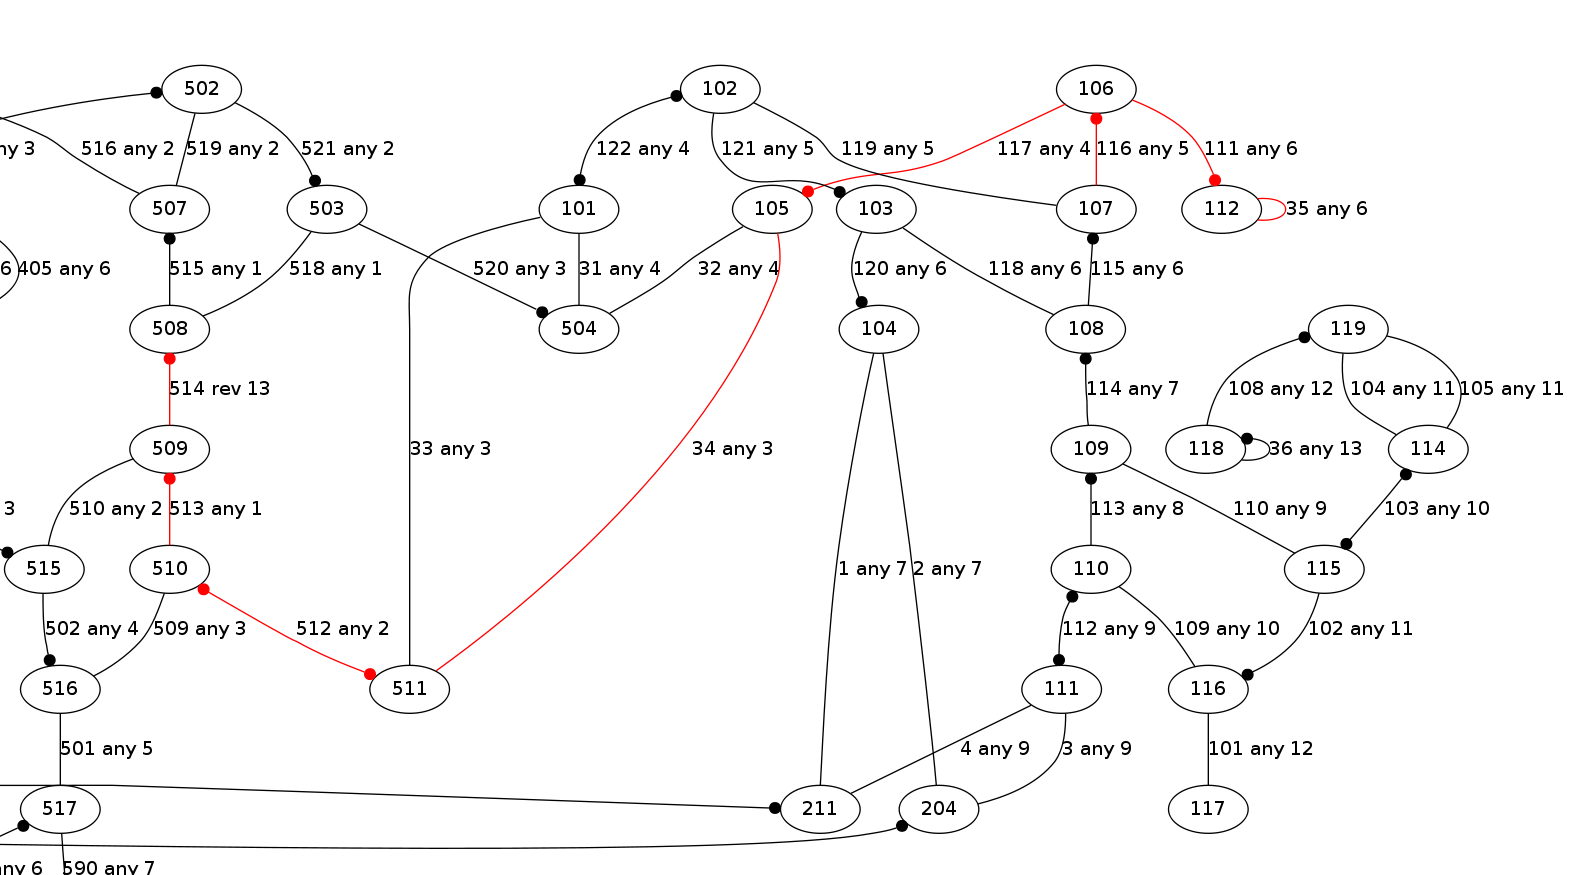
\includegraphics[width=7.5in]{reversing-514.png}
\caption{\label{fig:rev514}The path from segment 514 to the same segment with the train reversed. This also shows the points and segments involved in the 35 and 111 reversals.  }
\end{figure}
\begin{figure}
\centering
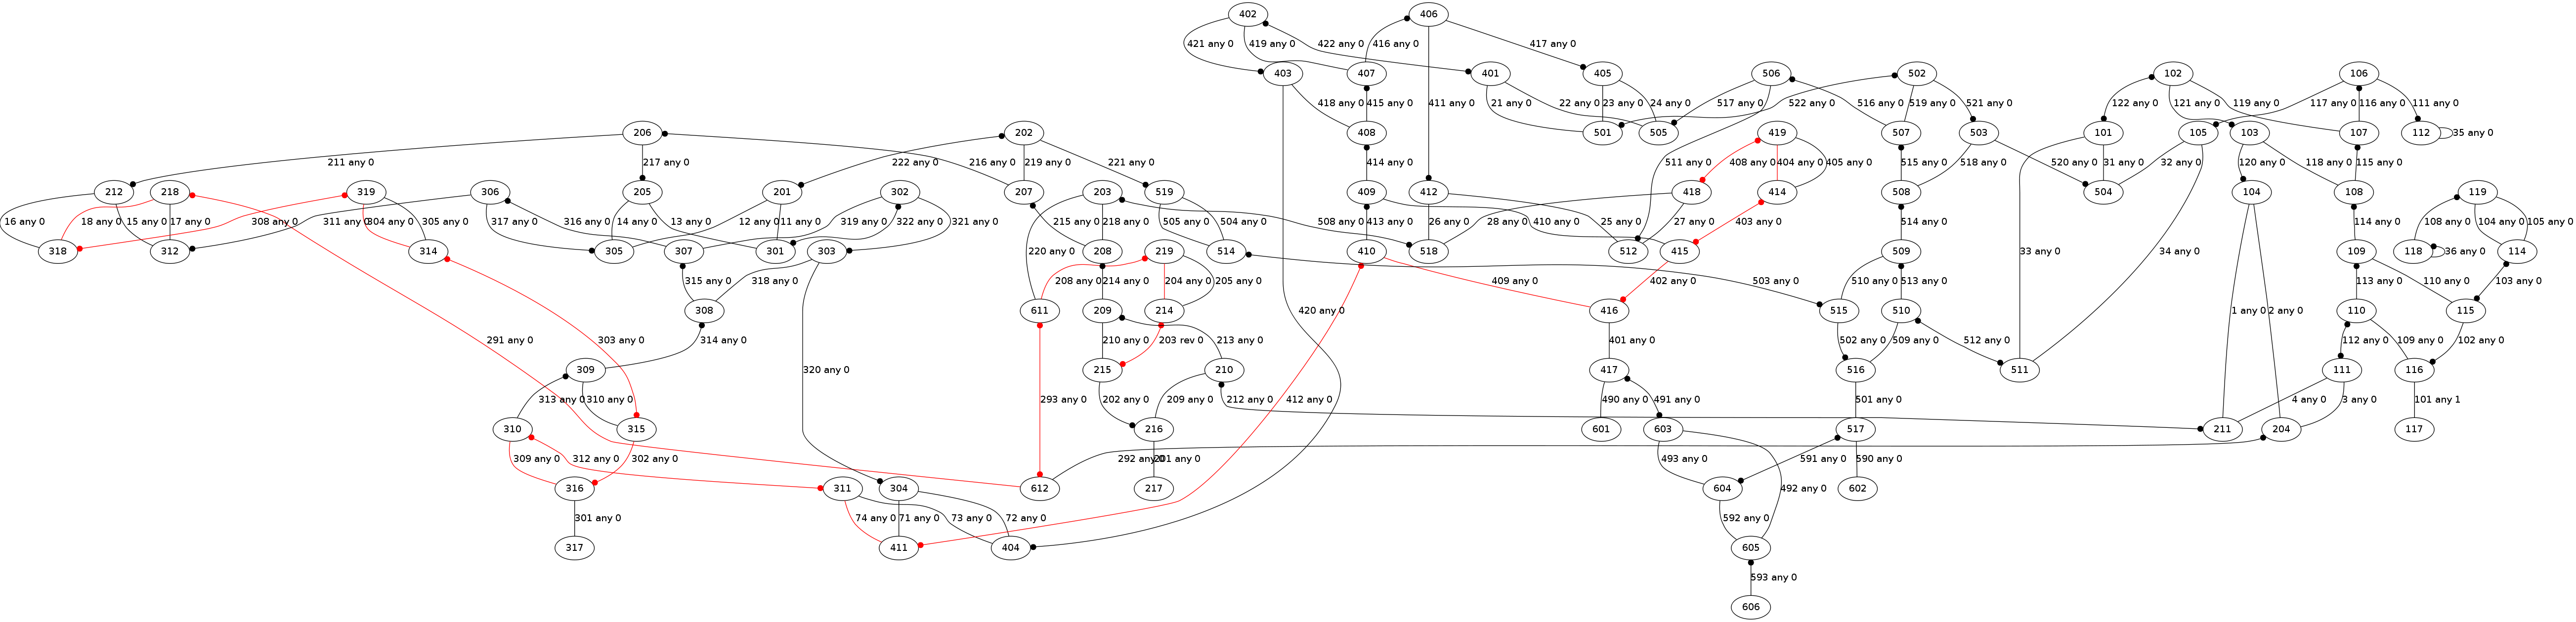
\includegraphics[width=7.5in]{path_203_408.png}
\caption{\label{fig:path}A minimal path from segment 203 to segment 408 minizing switch-backs. This also shows the entire rail network. }
\end{figure}

Both the rendered graphs (Figures \ref{fig:rev514} and \ref{fig:path}) and  are automatically generated by the software. We have complete graphs for every test we just don't have room for them. For smaller input sets we can also render the derived graph.

\end{document}